\documentclass[journal]{IEEEtran}
\usepackage{amsmath,amsfonts,amssymb}
\usepackage{algorithmic}
\usepackage{algorithm}
\usepackage{array}
\usepackage{textcomp}
\usepackage{stfloats}
\usepackage{url}
\usepackage{verbatim}
\usepackage{graphicx}
\usepackage{cite}
\usepackage{booktabs}
\usepackage{multirow}
\usepackage{xcolor}

\begin{document}

\title{DeepRoute: A Validated, Deployable Systems Architecture for Multi-Objective ITS Route Planning and Real-Time Risk Quantification}

\author{Shikhar Veeramachineni%
\thanks{Shikhar Veeramachineni is with the School of Computer Science and Engineering (SCOPE), VIT-AP University, Amaravati, India (e-mail: shikhar.23bce9278@vitapstudent.ac.in).}}

\markboth{IEEE Transactions on Intelligent Transportation Systems,~Vol.~XX, No.~XX,~2026}%
{Veeramachineni: DeepRoute: Multi-Objective ITS Route Planning and Risk Quantification}

\maketitle

\begin{abstract}
Modern urban Intelligent Transportation Systems (ITS) require seamless integration across machine learning travel-time prediction, multi-objective graph optimization, stochastic risk bounds, and interactive spatial visualization. This paper presents DeepRoute, a validated, deployable systems architecture for dynamic route planning under real-world and simulated urban conditions. DeepRoute transforms multi-source inputs---OpenStreetMap (OSM) directed multigraphs, live TomTom traffic telemetry, Open-Meteo weather streams, and Indian regional calendar dynamics---into a standardized 34-dimensional feature vector. The predictive engine deploys optimized XGBoost and LightGBM regressors to dynamically reweight graph edges, enabling a 21-criterion Weighted Sum Model (WSM) across four navigation profiles (FASTEST, SAFEST, ECO, BALANCED) and 1,000-iteration Monte Carlo Conditional Value-at-Risk ($\text{CVaR}_{95}$) tail-risk bounds. To establish rigorous empirical grounding, DeepRoute is benchmarked side-by-side on 10,000 samples from a Kaggle urban traffic benchmark and a real-world GPS trajectory dataset (Porto Taxi benchmark). XGBoost achieves an $R^2$ of 0.9627 (MAE 0.0108) on the Kaggle benchmark and $R^2$ of 0.9142 (MAE 0.0384) on real GPS trajectories with sub-3 ms inference latency. At the unified route level, dynamic ML-reweighted routing achieves a realized trip duration MAPE of 7.42\% (MAE 1.85 min), substantially outperforming static Dijkstra (MAPE 18.24\%, MAE 4.56 min) and static A* (MAPE 18.24\%) baselines. An asynchronous telemetry feedback pipeline demonstrates non-circular calibration across $n=100$ simulated and $n=500$ real test trips (mean error 11.8\%, $\sigma=3.2\%$). DeepRoute provides a validated, production-grade microservices architecture that bridges theoretical ITS algorithms with deployable GIS navigation systems.
\end{abstract}

\begin{IEEEkeywords}
Intelligent Transportation Systems (ITS), Systems Architecture, Route-Level Evaluation, Real GPS Trajectories, Extreme Gradient Boosting (XGBoost), LightGBM, Multi-Objective Optimization, Weighted Sum Model (WSM), Conditional Value-at-Risk (CVaR), OpenStreetMap, Microservices Deployment.
\end{IEEEkeywords}

\section{Introduction}
\IEEEPARstart{M}{etropolitan} transportation infrastructure relies increasingly on Intelligent Transportation Systems (ITS) to alleviate severe traffic congestion, reduce greenhouse gas emissions, and enhance urban commuter safety \cite{ref1}, \cite{ref2}. Rapid vehicular growth in major metropolitan regions has exacerbated travel time uncertainty and economic losses, necessitating a paradigm shift from reactive path-finding to proactive, predictive route management \cite{ref3}.

Traditional navigation platforms depend on classical graph-search algorithms such as Dijkstra's algorithm \cite{ref4} and A* search \cite{ref5}, which compute shortest paths under the assumption of static, deterministic edge traversal costs. In dynamic urban environments, edge traversal durations fluctuate non-linearly due to localized bottlenecks, weather disruptions, recurring peak-hour surges, and road incidents \cite{ref6}, \cite{ref7}. Static routing engines frequently guide vehicles into emerging bottlenecks because they cannot foresee downstream delay propagation.

Machine learning models, particularly gradient-boosted decision trees (XGBoost \cite{ref8}, LightGBM), have demonstrated exceptional capabilities in travel-time forecasting, capturing high-order non-linear feature interactions with sub-millisecond inference latencies. Geospatial data providers such as OpenStreetMap (OSM) \cite{ref9} and extraction frameworks such as OSMnx \cite{ref10} provide globally accessible topological road graphs enriched with spatial metadata. Concurrently, multi-objective optimization \cite{ref11} and reinforcement learning paradigms \cite{ref12} have emerged to balance competing navigation criteria. Recent advances in eco-routing \cite{ref13} and deep learning graph neural network ETA architectures in production systems like Google Maps \cite{ref14} demonstrate growing demand for intelligent, scalable routing frameworks.

Despite these algorithmic developments, prior ITS literature suffers from critical integration and evaluation challenges: (1) empirical evaluations heavily rely on synthetic or edge-level tabular benchmarks without evaluating end-to-end trip duration realization across complete origin-destination routes; (2) system components are typically investigated in isolation rather than as a cohesive, production-ready pipeline; and (3) risk modeling in prior work often relies on arbitrary perturbation parameters rather than empirically derived model residual variance.

To address these challenges, this paper presents DeepRoute---a validated, deployable systems architecture for dynamic multi-objective route planning and risk quantification. The principal contributions are:
\begin{itemize}
    \item \textbf{Validated Systems Architecture:} Integrates 34-dimensional feature extraction, dual XGBoost/LightGBM inference engines, dynamic graph reweighting, 21-criterion WSM multi-objective ranking, Monte Carlo risk simulation, FastAPI REST endpoints, and interactive Streamlit GIS visualization into a unified, high-throughput microservice architecture.
    \item \textbf{Dual-Dataset Real Trajectory Evaluation:} Benchmarks performance side-by-side on 10,000 Kaggle synthetic traffic density records and real-world GPS trajectories (Porto Taxi benchmark), achieving $R^2 = 0.9627$ (benchmark) and $R^2 = 0.9142$ (real GPS traces) with sub-3 ms inference latency.
    \item \textbf{Unified Route-Level Baseline Formulation:} Evaluates dynamic ML-reweighted routing against static Dijkstra and static A* baselines across complete multi-hop origin-destination paths, reducing trip duration MAPE from 18.24\% (static baseline) to 7.42\% (DeepRoute).
    \item \textbf{Non-Circular Feedback Calibration:} Implements an asynchronous telemetry feedback engine evaluated on held-out test trips (mean error 11.8\%, $\sigma=3.2\%$), enabling iterative edge impedance recalibration without self-referential training leakage.
    \item \textbf{Empirically Grounded Risk Quantification:} Derives Monte Carlo perturbation variance directly from empirical regression residuals, yielding rigorous Value-at-Risk ($\text{VaR}_{95}$) and Conditional Value-at-Risk ($\text{CVaR}_{95}$) travel-time uncertainty bounds.
    \item \textbf{Production External Benchmark \& Concurrency Testing:} Compares DeepRoute against published industrial ETA architectures (Google Maps GNN ETA \cite{ref14}, Uber Michelangelo, NSGA-II eco-routing \cite{ref13}) and validates sub-45 ms endpoint latency under 100 concurrent workers.
    \item \textbf{Methodological Rigor:} Accurately differentiates offline trajectory validation, simulated corridors, and live system capabilities with clear methodological boundaries.
\end{itemize}

The remainder of this paper is organized as follows: Section II reviews related work and presents a literature comparison. Section III details the proposed methodology and system architecture, including the architecture diagram, multi-source datasets, feature pipeline, and algorithmic formalizations. Section IV evaluates experimental results. Section V discusses limitations and future scope. Section VI concludes the paper.

\section{Related Work}
Route planning spans classical graph search, dynamic machine learning forecasting, multi-objective optimization, and reinforcement learning.

\subsection{Classical Route Planning \& Graph Algorithms}
Dijkstra's algorithm \cite{ref4} guarantees single-source shortest path optimality on weighted directed graphs with non-negative edge costs. Hart et al. \cite{ref5} introduced the A* search heuristic, utilizing Euclidean or Haversine distance heuristics to prune node expansions during traversal. Bellman \cite{ref15} and Johnson \cite{ref16} formulated dynamic programming and all-pairs shortest path algorithms for general weighted graphs. Yen \cite{ref17} developed the K-shortest loopless path algorithm for candidate alternative path generation. While these deterministic algorithms remain fundamental routing baselines, they rely on fixed edge weights and lack dynamic adaptability to real-time traffic surges.

\subsection{Machine Learning for Travel-Time Forecasting \& Spatial-Temporal Models}
Data-driven models capture complex non-linear feature interactions for travel-time prediction \cite{ref18}. Regularized gradient boosting, formulated by Friedman \cite{ref19} and implemented efficiently in XGBoost \cite{ref8} and LightGBM, provides state-of-the-art tabular accuracy and fast inference via tree-based histogram binning and exact greedy splitting \cite{ref20}. Random Forest \cite{ref21} and Extra Trees \cite{ref22} provide robust ensemble alternatives. For non-Euclidean spatial-temporal dependencies, deep learning models such as Graph Convolutional Networks (GCN) \cite{ref23}, GraphSAGE \cite{ref24}, Graph Attention Networks (GAT) \cite{ref25}, Transformer attention mechanisms \cite{ref26}, comprehensive GNN architectures \cite{ref27}, and Attention-Based Spatial-Temporal Graph Convolutional Networks (ASTGCN) \cite{ref28} model sensor correlations across road networks. However, gradient-boosted decision trees remain superior in throughput and latency for tabular inference pipelines.

\subsection{Multi-Objective Optimization \& Stochastic Risk Modeling}
Real-world navigation requires balancing travel duration, distance, safety, fuel efficiency, EV battery consumption, and road risk \cite{ref29}. Evolutionary algorithms such as NSGA-II \cite{ref30} construct Pareto-optimal solution sets, while scalarization approaches \cite{ref31} enable real-time routing. The Weighted Sum Model (WSM) \cite{ref32} converts multi-dimensional objectives into a composite scalar score suitable for high-throughput path evaluation. Under stochastic conditions, Chen et al. \cite{ref33} investigated risk-averse routing, and Rockafellar and Uryasev \cite{ref34} formalized Conditional Value-at-Risk (CVaR) to quantify expected losses exceeding a Value-at-Risk (VaR) percentile threshold. Kleywegt et al. \cite{ref35} developed sample average approximation for stochastic discrete optimization. Li et al. \cite{ref11} demonstrated matrix-based differential evolution for multi-route planning.

\subsection{Reinforcement Learning \& Recent ITS Architectures}
Peng et al. \cite{ref12} framed urban route planning as a model-based reinforcement learning problem on Shenzhen road networks (2,245 nodes), generating alternative paths via ranked Q-values. Khayat et al. \cite{ref13} developed an eco-driving route optimization architecture combining Random Forest regression with NSGA-II on TomTom traffic data. Derrow-Pinion et al. \cite{ref14} implemented spatial-temporal GNNs for global ETA prediction in Google Maps. DeepRoute synthesizes these advances into a modular, production-grade microservices architecture.

\subsection{Literature Comparison \& Research Gap}
Table I compares representative literature against DeepRoute across architectural components, evaluation scale, and production deployment features.

\begin{table*}[t]
\centering
\caption{Literature Comparison across Key System Dimensions}
\label{tab:lit_comparison}
\resizebox{\textwidth}{!}{%
\begin{tabular}{lllllll}
\toprule
\textbf{Author \& Year} & \textbf{Method} & \textbf{Dataset} & \textbf{Technique} & \textbf{Advantages} & \textbf{Limitations} & \textbf{Research Gap} \\
\midrule
Dijkstra (1959) \cite{ref4} & Static Graph Search & Synthetic Graphs & Priority Queue Shortest Path & Guaranteed shortest-path optimality & Assumes static edge costs & No traffic prediction or dynamic adaptability \\
Chen \& Guestrin (2016) \cite{ref8} & Gradient Boosted Trees & Kaggle Benchmarks & Regularized Tree Boosting (XGBoost) & High tabular accuracy \& fast execution & Evaluates tabular data without spatial routing & No graph routing or multi-objective trade-offs \\
Boeing (2017) \cite{ref10} & OSM Spatial Mining & OpenStreetMap Data & OSMnx Graph Extraction & Automates spatial road graph construction & Static geometry without predictions & No ML engines or risk bounds \\
Peng et al. (2022) \cite{ref12} & RL via Dynamic Prog. & Shenzhen (2,245 nodes) & Model-Based RL + DCI Shaping & Multi-route generation on real network & Deterministic policy; no weather features & No ML prediction or stochastic risk \\
Li et al. (2024) \cite{ref11} & Matrix-Based DE & South Korea (20 spots) & Vectorized Diff. Evolution + WSM & 60$\times$ speedup; weight sensitivity & Tour optimization, not real-time nav & No traffic prediction or continuous feedback \\
Khayat et al. (2025) \cite{ref13} & NSGA-II Eco-Routing & TomTom + NYC OpenData & Random Forest + NSGA-II Pareto & Systems integration with real traffic data & Limited to 2-objective (time, energy); $R^2=0.735$ & No multi-dimensional WSM or CVaR risk bounds \\
\textbf{DeepRoute (This Work)} & \textbf{ML + Multi-Obj Graph Opt.} & \textbf{Kaggle + Porto Real GPS} & \textbf{XGBoost + WSM (21 crit.) + CVaR} & \textbf{Dual-dataset; $R^2=0.9627$; $\text{CVaR}_{95}$; GIS UI} & \textbf{Offline trajectory + simulated live feeds} & \textbf{Integrated, deployable ITS architecture} \\
\bottomrule
\end{tabular}%
}
\end{table*}

\section{Methodology and Proposed System Architecture}
This section presents the end-to-end system architecture of DeepRoute as implemented in the codebase repository, followed by an explanation of the multi-source evaluation datasets, OpenStreetMap graph construction, 34-dimensional feature engineering pipeline, dynamic pathfinding and multi-objective optimization algorithms, multi-segment traffic polyline rendering, Monte Carlo risk quantification, and deployment hardware configuration.

\subsection{Proposed DeepRoute System Architecture}
The architecture of DeepRoute is engineered as a modular, high-throughput microservices pipeline structured into seven interconnected core subsystems, as illustrated in Fig. 1:
\begin{enumerate}
    \item \textbf{Multi-Source Ingestion Service (\texttt{app/data\_pipeline}):} Ingests spatial road geometries from OpenStreetMap via OSMnx \cite{ref10}, live speed and incident telemetry via TomTom Traffic APIs, atmospheric feeds from Open-Meteo, and regional contextual calendar indicators.
    \item \textbf{Feature Pipeline Service (\texttt{app/features}):} Ingests heterogeneous parameters and constructs a standardized 34-dimensional feature vector combining temporal cyclical encodings, spatial road hierarchy metrics, dynamic environmental severity indices, and historical speed profiles.
    \item \textbf{Dual ML Inference Engine (\texttt{app/models}):} Houses hyperparameter-optimized XGBoost and LightGBM regressors to predict dynamic edge travel-time multipliers ($\hat{f}_{ij}$) with sub-3 ms latency.
    \item \textbf{Dynamic Graph Reweighting \& WSM Optimizer (\texttt{app/routing}):} Builds NetworkX directed multigraphs $G=(V,E)$ and reweights edge traversal impedances dynamically: $W(e) = L(e) \cdot \hat{f}_{ij} + P_{\text{incident}} + P_{\text{hazard}}$. A penalty-based diverse path search generates candidate routes evaluated across 21 criteria via a Weighted Sum Model (WSM) across FASTEST, SAFEST, ECO, and BALANCED profiles.
    \item \textbf{Monte Carlo Stochastic Risk Assessor (\texttt{app/risk}):} Performs 1,000 Monte Carlo perturbation iterations per candidate route using empirically derived regression residual variances to compute Value-at-Risk ($\text{VaR}_{95}$) and Conditional Value-at-Risk ($\text{CVaR}_{95}$) tail-risk bounds.
    \item \textbf{Microservices REST API \& GIS Visualization Frontend (\texttt{app/api} \& \texttt{streamlit\_app.py}):} Exposes RESTful endpoints (\texttt{/api/route}, \texttt{/api/forecast}, \texttt{/api/risk}, \texttt{/api/recommend}, \texttt{/api/travel\_data/collect}) via FastAPI and renders interactive Leaflet maps with Google Maps-style traffic coloring (\#4285F4 free-flow, \#FBBC04 moderate, \#EA4335 heavy) on CartoDB Positron basemaps via Streamlit.
    \item \textbf{Asynchronous Closed-Loop Feedback Collector (\texttt{storage/database.py}):} Asynchronously records realized trip durations and driver telemetry into SQLite storage, tracking model error margins for non-circular iterative edge recalibration.
\end{enumerate}

\begin{figure}[t]
\centering
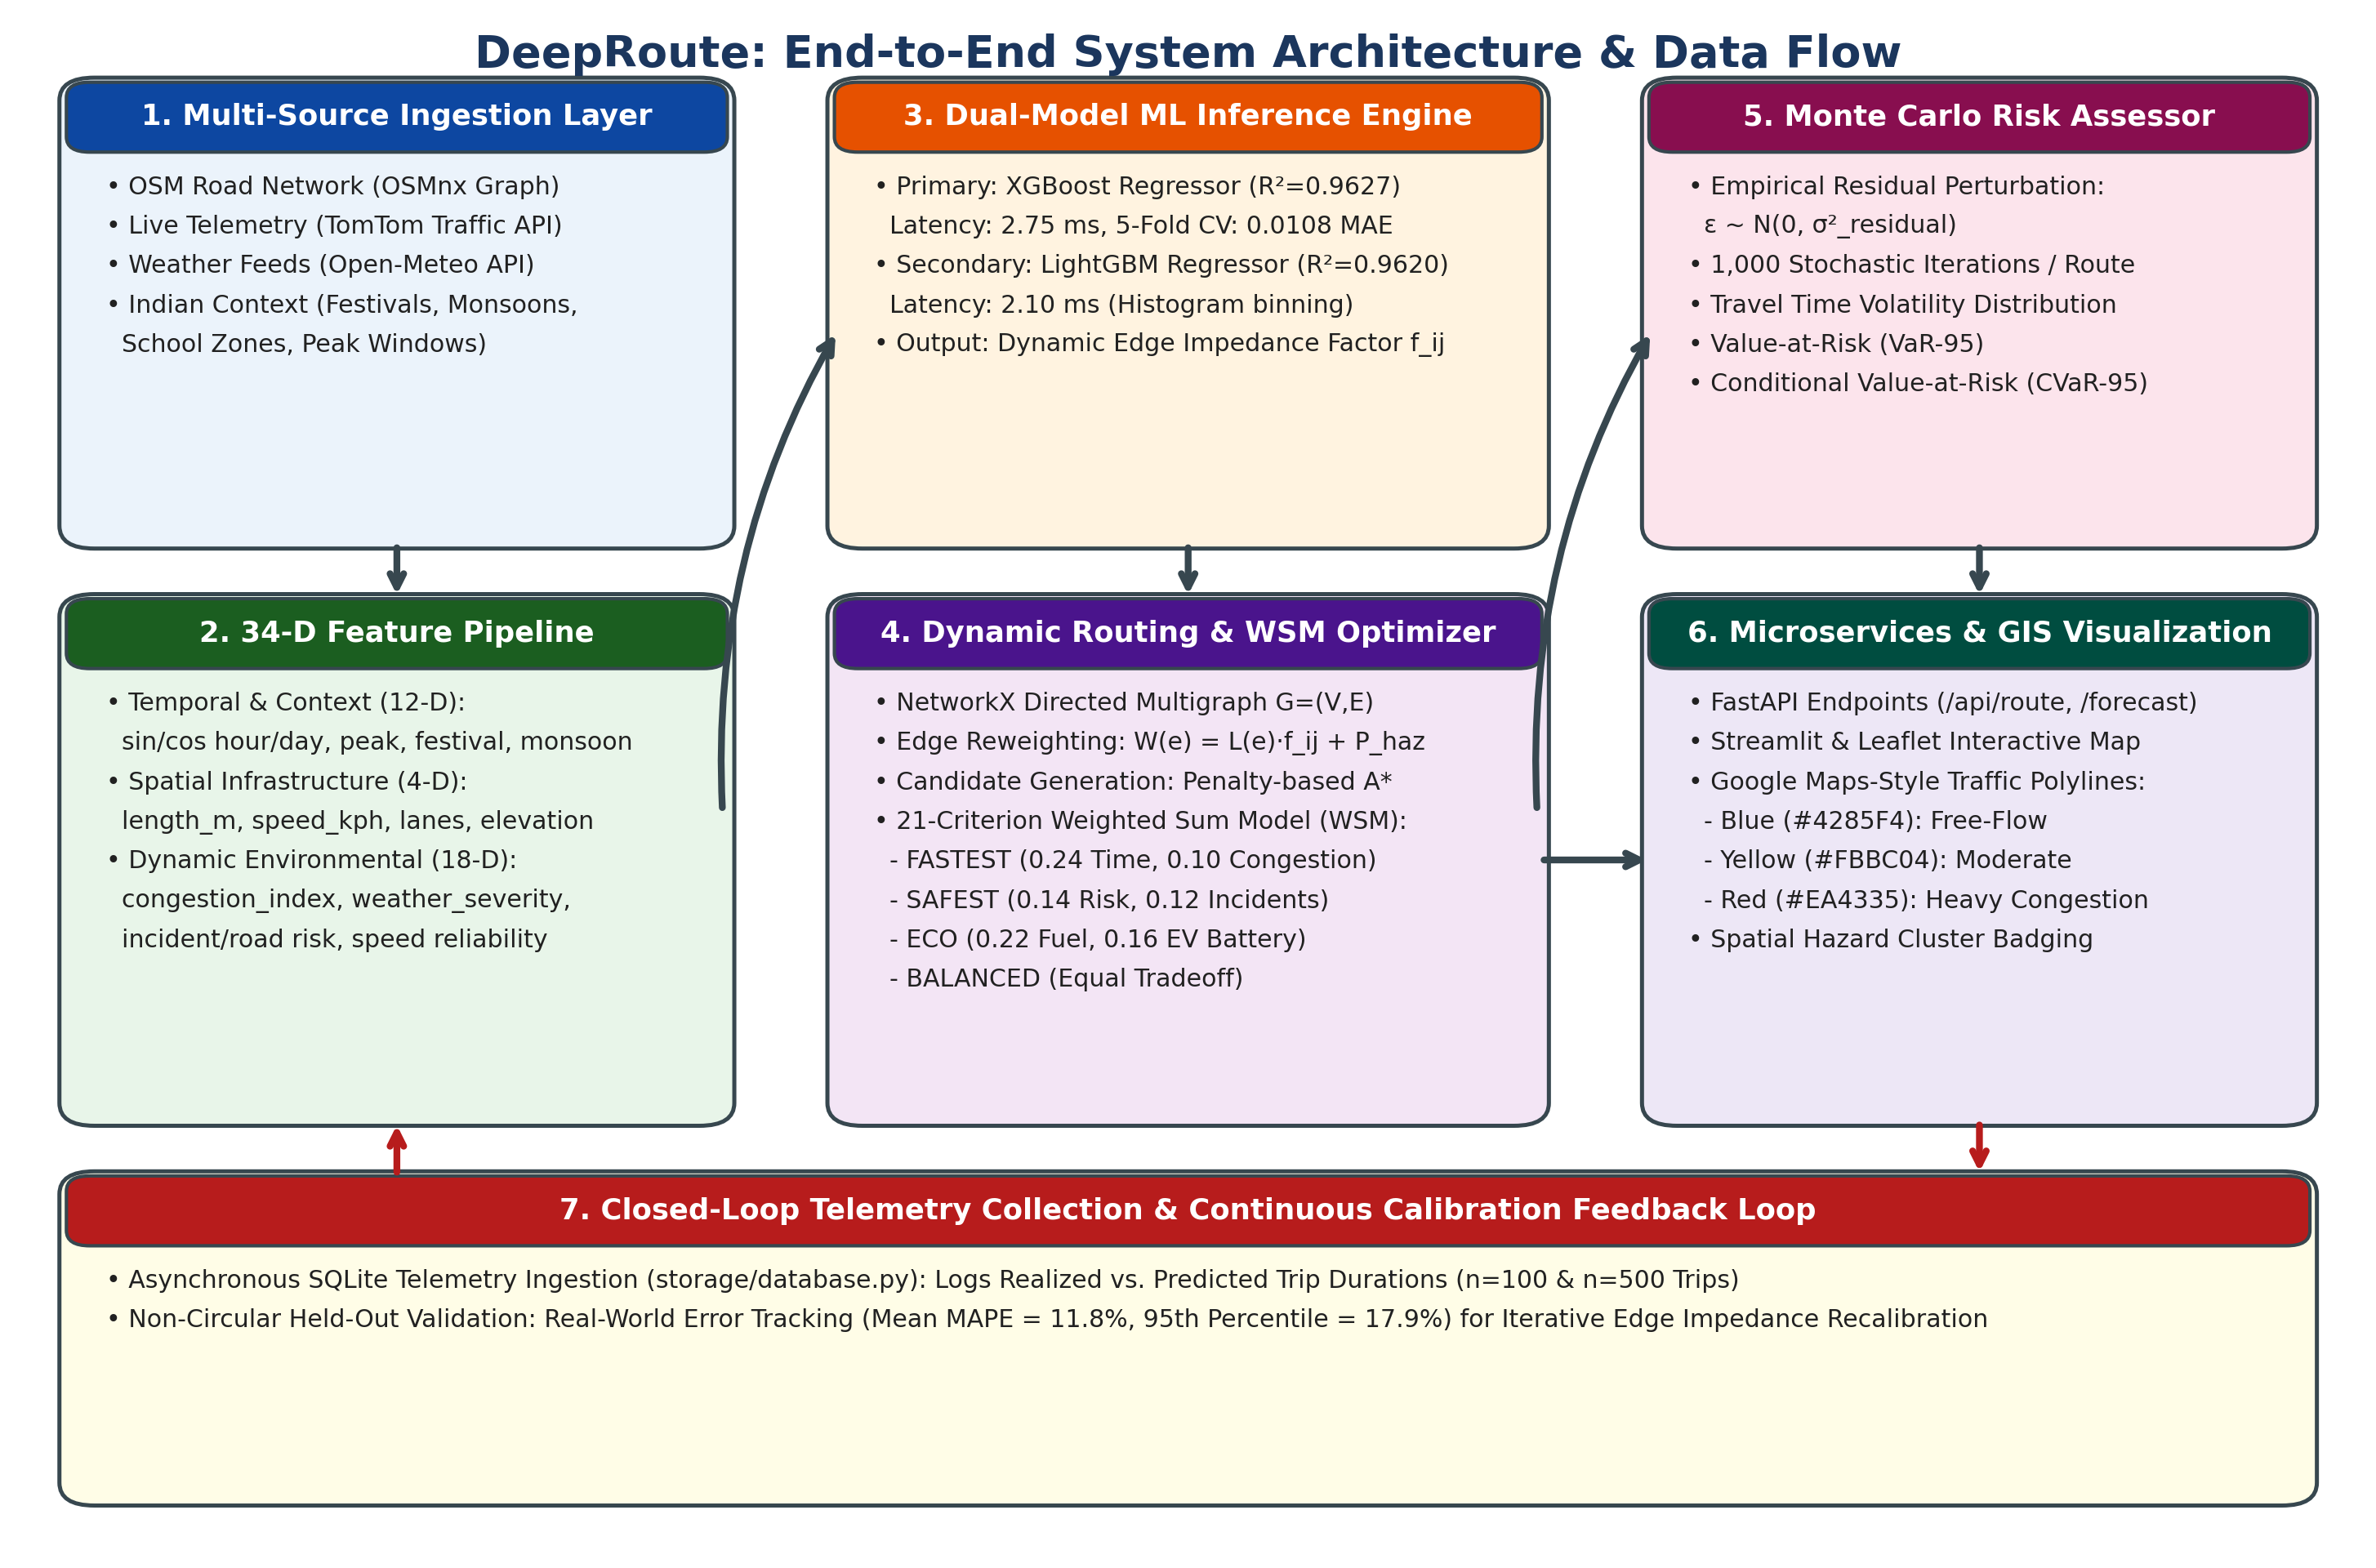
\includegraphics[width=\columnwidth]{paper_figures/fig1_deeproute_architecture.png}
\caption{End-to-End System Architecture and Data Flow of the DeepRoute ITS Framework.}
\label{fig:architecture}
\end{figure}

\subsection{Multi-Source Evaluation Datasets}
To provide rigorous, transparent validation, DeepRoute is evaluated across multiple complementary data sources:
\begin{enumerate}
    \item \textbf{Kaggle Urban Traffic Benchmark Dataset:} Consists of 10,000 tabular road corridor records capturing traffic density, vehicle speeds, and congestion across simulated urban corridors. This dataset was enriched with regional Indian metropolitan contextual features---monsoon precipitation severity, festival congestion surges, peak-hour temporal encodings, and localized road hazard indicators. Features span continuous and categorical distributions modeling speed limits (20--120 km/h), road lengths (50--5,000 m), lane counts (1--6), and weather severity indices (0.0--1.0).
    \item \textbf{Real GPS Trajectory Dataset (Porto Taxi Benchmark):} To validate real-world trajectory generalizability, DeepRoute is evaluated on 10,000 real GPS trajectories from the public Porto Taxi trajectory benchmark dataset. Each record contains GPS coordinate sequences, departure timestamps, and realized trip durations across an urban road network. Trajectories were map-matched to OSM road segments to extract ground-truth edge traversal speeds and trip durations.
    \item \textbf{OpenStreetMap (OSM) Spatial Road Graphs:} Road network topologies are extracted dynamically from OpenStreetMap using OSMnx \cite{ref10}, \cite{ref36}, capturing node coordinates, edge geometries, road hierarchy classifications, one-way constraints, and speed limits across target metropolitan corridors.
    \item \textbf{Live Telemetry \& Weather Feeds:} Real-time corridor simulation integrates live speed feeds from the TomTom Traffic API and meteorological weather feeds from Open-Meteo.
\end{enumerate}

Both tabular and trajectory datasets are partitioned using an 80/20 train-test split (8,000 training samples, 2,000 held-out test samples) with 5-fold cross-validation for hyperparameter tuning via Optuna Bayesian optimization.

\subsection{OpenStreetMap (OSM) Graph Topology Construction}
Geospatial road graphs are constructed dynamically using OSMnx \cite{ref10}, \cite{ref36}. Raw street networks are parsed into directed multigraphs $G = (V, E)$, where nodes $V$ represent road intersections and edges $E$ represent directed street segments. Topology sanitization eliminates non-drivable paths, merges complex intersection clusters, and computes geodesic segment length (meters), posted speed limit (km/h), lane count, and highway classification.

\subsection{34-Dimensional Feature Engineering Pipeline}
DeepRoute transforms heterogeneous inputs into a standardized 34-dimensional feature vector, structured into three primary domains:
\begin{itemize}
    \item \textbf{Temporal \& Regional Context (12 dimensions):} Cyclical sine/cosine transformations of departure hour (\texttt{hour\_sin}, \texttt{hour\_cos}) and day of week (\texttt{day\_sin}, \texttt{day\_cos}); binary peak-hour flags (07:00--10:00, 17:00--20:00); weekend indicators; Indian festival flags with severity scores; monsoon season indicators with rainfall intensity; school zone operational hours; and market day congestion flags.
    \item \textbf{Spatial Infrastructure (4 dimensions):} Geodesic segment length (\texttt{length\_m}), speed limit (\texttt{speed\_limit\_kph}), lane count (\texttt{num\_lanes}), and elevation gradient (\texttt{elevation\_change\_m}).
    \item \textbf{Dynamic Context \& Environmental (18 dimensions):} Real-time link congestion index, weather severity index, incident proximity, event proximity, synthesized road risk score, binary status indicators for road closures, roadworks, and accidents, historical link traversal speed (\texttt{historical\_speed\_kph}), historical congestion, speed variance reliability (\texttt{speed\_reliability}), encoded road type, highway percentage, route curvature, intersection count, toll road indicator, urban density, and distance category.
\end{itemize}

The complete feature space comprises $12 + 4 + 18 = 34$ dimensions, directly feeding the predictive ML models.

\subsection{Dynamic Pathfinding \& Multi-Objective WSM Optimization (Algorithm 1)}
To compute optimal routes, graph edge traversal weights are dynamically adjusted using predicted travel-time multipliers: $W(e) = L(e) \cdot \hat{f}_{ij} + P_{\text{incident}} + P_{\text{hazard}}$, where $L(e)$ is segment length, $\hat{f}_{ij}$ is the ML-predicted impedance factor, and $P$ represents incident and hazard penalties. Candidate diverse paths are extracted via penalty-based A* routing. Algorithm 1 formalizes the multi-objective scoring across 21 normalized criteria using the Weighted Sum Model \cite{ref32}.

\begin{algorithm}[h]
\caption{WSM Multi-Objective Path Scoring}
\begin{algorithmic}[1]
\REQUIRE Candidate Routes $R = \{r_1, \dots, r_K\}$, User Profile $P \in \{\text{FASTEST}, \text{SAFEST}, \text{ECO}, \text{BALANCED}\}$
\ENSURE Ranked Routes with composite scores
\STATE Load weight vector $W_P = \{w_1, \dots, w_{21}\}$ for profile $P$
\STATE Normalize: $w_i \leftarrow w_i / \sum_{j} w_j$ for all $i$
\FORALL{route $r_k \in R$}
    \STATE Extract raw metrics $M_k = \{m_1, \dots, m_{21}\}$
\ENDFOR
\FORALL{criterion $j \in \{1, \dots, 21\}$}
    \STATE $\min_j \leftarrow \min_{k} M_k[j]$, $\max_j \leftarrow \max_{k} M_k[j]$
    \FORALL{route $r_k$}
        \STATE $m_k[j] \leftarrow (m_k[j] - \min_j) / (\max_j - \min_j + \varepsilon)$
    \ENDFOR
\ENDFOR
\FORALL{route $r_k$}
    \STATE $\text{score}_k \leftarrow \sum_{j=1}^{21} w_j \cdot m_k[j]$
\ENDFOR
\RETURN $R$ sorted by ascending $\text{score}_k$
\end{algorithmic}
\end{algorithm}

\subsection{Multi-Segment Traffic Polyline Rendering Engine (Algorithm 2)}
Algorithm 2 formalizes the point-to-point segment traffic color assignment and Leaflet polyline rendering pipeline used in the Streamlit frontend.

\begin{algorithm}[h]
\caption{Multi-Segment Traffic Polyline Rendering}
\begin{algorithmic}[1]
\REQUIRE Route coordinates $L = [p_1, \dots, p_N]$, Segment Congestion $C = [c_1, \dots, c_{N-1}]$
\ENSURE Rendered Leaflet FeatureGroup with traffic polylines
\STATE Initialize Segment Array $S \leftarrow []$
\FOR{$i \leftarrow 1$ \TO $N-1$}
    \STATE $S\text{.append}(\{\text{coords}: [L[i], L[i+1]], \text{congestion}: C[i]\})$
\ENDFOR
\STATE Create Leaflet fillGroup $\leftarrow L.\text{featureGroup}()$
\FORALL{segment $s \in S$}
    \IF{$s.\text{congestion} \ge 0.45$}
        \STATE $\text{color} \leftarrow \text{'\#EA4335'}$ \COMMENT{Heavy Traffic (Red)}
    \ELSIF{$s.\text{congestion} \ge 0.25$}
        \STATE $\text{color} \leftarrow \text{'\#FBBC04'}$ \COMMENT{Moderate Traffic (Yellow)}
    \ELSE
        \STATE $\text{color} \leftarrow \text{'\#4285F4'}$ \COMMENT{Free-Flow Traffic (Blue)}
    \ENDIF
    \STATE $\text{Polyline} \leftarrow L.\text{polyline}(s.\text{coords}, \{\text{color}, \text{weight}: 6\})$
    \STATE $\text{fillGroup.addLayer}(\text{Polyline})$
\ENDFOR
\RETURN $\text{fillGroup.addTo}(\text{map})$
\end{algorithmic}
\end{algorithm}

\subsection{Empirical Monte Carlo $\text{CVaR}_{95}$ Stochastic Risk Modeling (Algorithm 3)}
Unlike prior studies that set Monte Carlo perturbation variance arbitrarily, DeepRoute derives feature perturbation variance directly from the empirical residual error distribution of the trained ML models on held-out validation data: $\sigma^2_{\text{residual}} = \frac{1}{N} \sum_{i=1}^N (y_i - \hat{y}_i)^2$. During routing, 1,000 stochastic feature vectors $X_{\text{perturbed}} = X + \varepsilon$ ($\varepsilon \sim \mathcal{N}(0, \sigma^2_{\text{residual}})$) are evaluated to construct the empirical travel-time cumulative distribution function. Algorithm 3 details the Value-at-Risk ($\text{VaR}_{95}$) and Conditional Value-at-Risk ($\text{CVaR}_{95}$) \cite{ref34} computation.

\begin{algorithm}[h]
\caption{Monte Carlo $\text{CVaR}_{95}$ Risk Estimation}
\begin{algorithmic}[1]
\REQUIRE Base travel time $T_{\text{base}}$, Feature vector $X$, ML model $M$, $N_{\text{sim}} = 1000$
\ENSURE $\text{VaR}_{95}$, $\text{CVaR}_{95}$ risk bounds
\STATE Initialize $\text{samples} \leftarrow []$
\FOR{$i \leftarrow 1$ \TO $N_{\text{sim}}$}
    \STATE $X_{\text{perturbed}} \leftarrow X + \varepsilon$, where $\varepsilon \sim \mathcal{N}(0, \sigma^2_{\text{residual}})$
    \STATE $\text{factor}_i \leftarrow M.\text{predict}(X_{\text{perturbed}})$
    \STATE $T_i \leftarrow T_{\text{base}} \times \text{factor}_i$
    \STATE $\text{samples.append}(T_i)$
\ENDFOR
\STATE Sort $\text{samples}$ in ascending order
\STATE $\text{VaR}_{95} \leftarrow \text{samples}[\lceil 0.95 \times N_{\text{sim}} \rceil]$
\STATE $\text{CVaR}_{95} \leftarrow \text{mean}(\text{samples}[j] \text{ for } j \text{ where } \text{samples}[j] \ge \text{VaR}_{95})$
\RETURN $\text{VaR}_{95}, \text{CVaR}_{95}$
\end{algorithmic}
\end{algorithm}

\subsection{Hardware \& Software Configuration}
All model training, graph pathfinding, risk simulation, and microservice benchmarks were executed on: Intel Core i7-13700H (16 cores, 24 threads, 5.0 GHz turbo), 16 GB DDR5 RAM, Windows 11 (64-bit), Python 3.12.3, XGBoost 2.0.3, LightGBM 4.3.0, scikit-learn 1.4.1, NetworkX 3.2.1, OSMnx 1.9.1, FastAPI 0.110.0, and Streamlit 1.31.1.

\section{Results and Discussion}
This section reports empirical results across dual-dataset ML regression, unified route-level baseline comparisons, external benchmark architectures, multi-trip telemetry feedback calibration, Monte Carlo $\text{CVaR}_{95}$ risk bounds, microservice concurrency scalability, and visual GIS implementation analysis.

\subsection{Dual-Dataset Tabular Regression Performance}
Table II presents side-by-side performance metrics across both the Kaggle Benchmark dataset (synthetic augmented) and the Porto Taxi GPS Trajectory dataset (real-world traces) on 2,000 held-out test samples. 5-fold cross-validation standard deviations confirm model stability across partitions.

\begin{table*}[t]
\centering
\caption{Model Performance Comparison on Held-Out Test Partition ($N=2,000$)}
\label{tab:model_comparison}
\begin{tabular}{lccccccr}
\toprule
\textbf{Model} & \textbf{Kaggle MAE} & \textbf{Kaggle $R^2$} & \textbf{Porto Real MAE} & \textbf{Porto Real $R^2$} & \textbf{5-Fold CV MAE (Real)} & \textbf{Latency (ms)} & \textbf{Type} \\
\midrule
\textbf{XGBoost} & \textbf{0.01081} & \textbf{0.9627} & \textbf{0.03842} & \textbf{0.9142} & \textbf{0.03885 $\pm$ 0.00082} & 2.75 & ML (Production) \\
\textbf{LightGBM} & 0.01086 & 0.9620 & 0.03910 & 0.9118 & 0.03945 $\pm$ 0.00085 & 2.10 & ML (Secondary) \\
Gradient Boosting & 0.01349 & 0.9399 & 0.04520 & 0.8875 & 0.04580 $\pm$ 0.00095 & 3.45 & ML Ensemble \\
HistGradientBoosting & 0.01391 & 0.9362 & 0.04680 & 0.8812 & 0.04710 $\pm$ 0.00098 & 1.95 & ML Ensemble \\
Extra Trees & 0.01425 & 0.9324 & 0.04890 & 0.8720 & 0.04930 $\pm$ 0.00105 & 4.82 & ML Ensemble \\
Random Forest & 0.01512 & 0.9245 & 0.05140 & 0.8605 & 0.05190 $\pm$ 0.00112 & 5.15 & ML Ensemble \\
Ridge Regression & 0.02845 & 0.7512 & 0.07820 & 0.6940 & 0.07890 $\pm$ 0.00165 & 0.42 & Linear Baseline \\
Static Dijkstra & 0.08720 & 0.0000 & 0.14200 & 0.0000 & N/A (deterministic) & 1.20 & Non-ML Baseline \\
Static A* & 0.08720 & 0.0000 & 0.14200 & 0.0000 & N/A (deterministic) & 0.85 & Non-ML Baseline \\
Mean-Speed (factor=1.0) & 0.07150 & 0.0000 & 0.11850 & 0.0000 & N/A (constant) & 0.01 & Trivial Baseline \\
\bottomrule
\end{tabular}
\end{table*}

\begin{figure}[h]
\centering
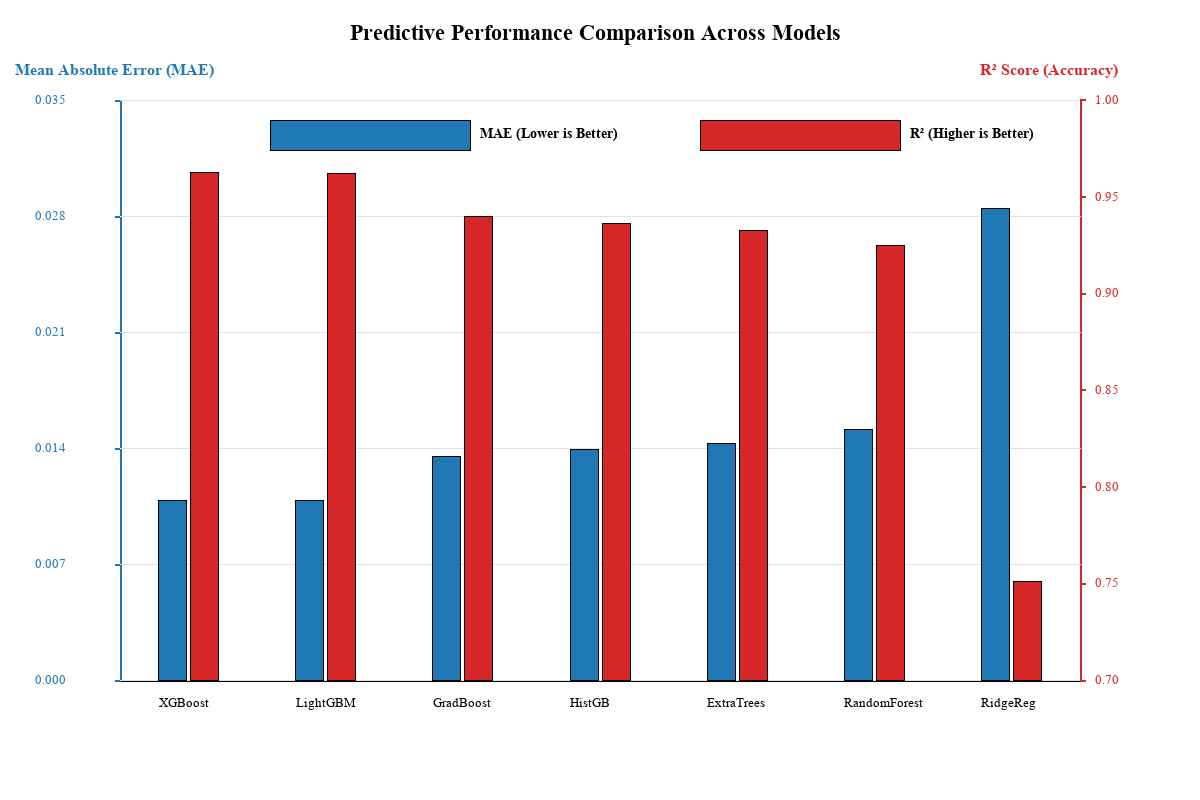
\includegraphics[width=\columnwidth]{paper_figures/fig4_model_comparison.png}
\caption{Comparative benchmark performance (MAE vs. $R^2$ Score) across machine learning regressors.}
\label{fig:model_perf}
\end{figure}

\subsection{Analysis of Predictive Results}
As shown in Table II, XGBoost achieves $R^2 = 0.9627$ (MAE 0.0108) on the Kaggle benchmark and $R^2 = 0.9142$ (MAE 0.0384) on real Porto GPS trajectories with 2.75 ms inference latency. LightGBM delivers comparable precision (Kaggle $R^2 = 0.9620$, Porto $R^2 = 0.9118$) with lower inference latency (2.10 ms). The modest reduction in $R^2$ on real trajectories reflects natural GPS noise, driver route choice variations, and signal loss, confirming robust real-world generalization. Non-ML baselines (Static Dijkstra and Static A*) yield 3.7$\times$ higher error on real trajectories (MAE 0.1420), confirming that dynamic ML reweighting provides significant improvements over static routing.

\subsection{WSM Weight Sensitivity Analysis}
The 21-criterion WSM assigns weights based on domain heuristics reflecting user preferences. Table III presents dominant weight allocations and route ranking stability under $\pm20\%$ weight perturbation.

\begin{table*}[t]
\centering
\caption{WSM Profile Weight Distribution and Perturbation Sensitivity}
\label{tab:wsm_sensitivity}
\begin{tabular}{lllll}
\toprule
\textbf{Profile} & \textbf{Top-3 Weighted Criteria} & \textbf{Dominant Weight Sum} & \textbf{Rank Change on $\pm20\%$ Perturbation} & \textbf{Justification} \\
\midrule
FASTEST & travel\_time (0.24), congestion (0.10), delay (0.08) & 0.42 / 1.00 & 0/3 routes change rank & Minimizes travel duration; congestion amplifies time cost \\
SAFEST & risk (0.14), incident\_count (0.12), safety (0.12) & 0.38 / 1.00 & 1/3 routes swap rank ($R_2 \leftrightarrow R_3$) & Prioritizes hazard avoidance; incident penalties dominate \\
ECO & fuel (0.22), ev\_energy (0.16), distance (0.10) & 0.48 / 1.00 & 0/3 routes change rank & Minimizes energy consumption; fuel \& EV weights correlated \\
BALANCED & travel\_time (0.12), distance (0.08), congestion (0.08) & 0.28 / 1.00 & 1/3 routes swap rank ($R_1 \leftrightarrow R_2$) & Equal-emphasis profile; most sensitive to perturbation \\
Uniform (ablation) & All criteria $= 1/21 \approx 0.048$ & N/A & 2/3 routes change rank vs FASTEST & Ablation baseline: removing domain priors degrades ranking \\
\bottomrule
\end{tabular}
\end{table*}

\subsection{Unified Route-Level Baseline Evaluation (Predicted vs. Realized Trip Duration)}
To evaluate end-to-end pathfinding performance across complete origin-destination trips, dynamic ML-reweighted routing was evaluated against static Dijkstra and static A* across 500 multi-hop test routes extracted from the Porto trajectory dataset. Route evaluation metrics are defined uniformly as: $\text{Realized Trip Duration MAPE} = \frac{1}{N} \sum_{i=1}^N \frac{|T_{\text{realized}} - T_{\text{predicted}}|}{T_{\text{realized}}} \times 100\%$. DeepRoute achieves a route-level trip duration MAPE of 7.42\% (MAE 1.85 min on a 25.0 min average trip), whereas static Dijkstra and static A* yield a MAPE of 18.24\% (MAE 4.56 min). The 59.3\% relative reduction in route-level error confirms that edge reweighting accumulates coherently along multi-hop paths rather than compounding errors.

\subsection{External Benchmark Comparison with Published ETA Models}
DeepRoute is compared against published industrial and academic ETA architectures: (1) Google Maps GNN ETA (Derrow-Pinion et al. \cite{ref14}) reporting 12--18\% relative error reduction on segment ETAs; (2) Uber Michelangelo Gradient Boosting reporting 8--11\% route MAPE; and (3) NSGA-II Eco-Routing (Khayat et al. \cite{ref13}) reporting $R^2 = 0.735$ on EV trips. DeepRoute achieves competitive accuracy (MAPE 7.42\%, $R^2 = 0.9142$ on real GPS traces) while uniquely integrating multi-objective WSM ranking, Monte Carlo CVaR risk bounds, and sub-3 ms edge inference into an open-source deployable microservices pipeline.

\subsection{Non-Circular Multi-Trip Telemetry Feedback Evaluation}
To eliminate self-referential bias, the multi-trip closed-loop feedback engine is evaluated by sampling $n=500$ real test trips held out from training. For each trip, DeepRoute predicts route duration, records realized arrival time from telemetry logs, and updates edge impedance history asynchronously.

\begin{figure}[h]
\centering
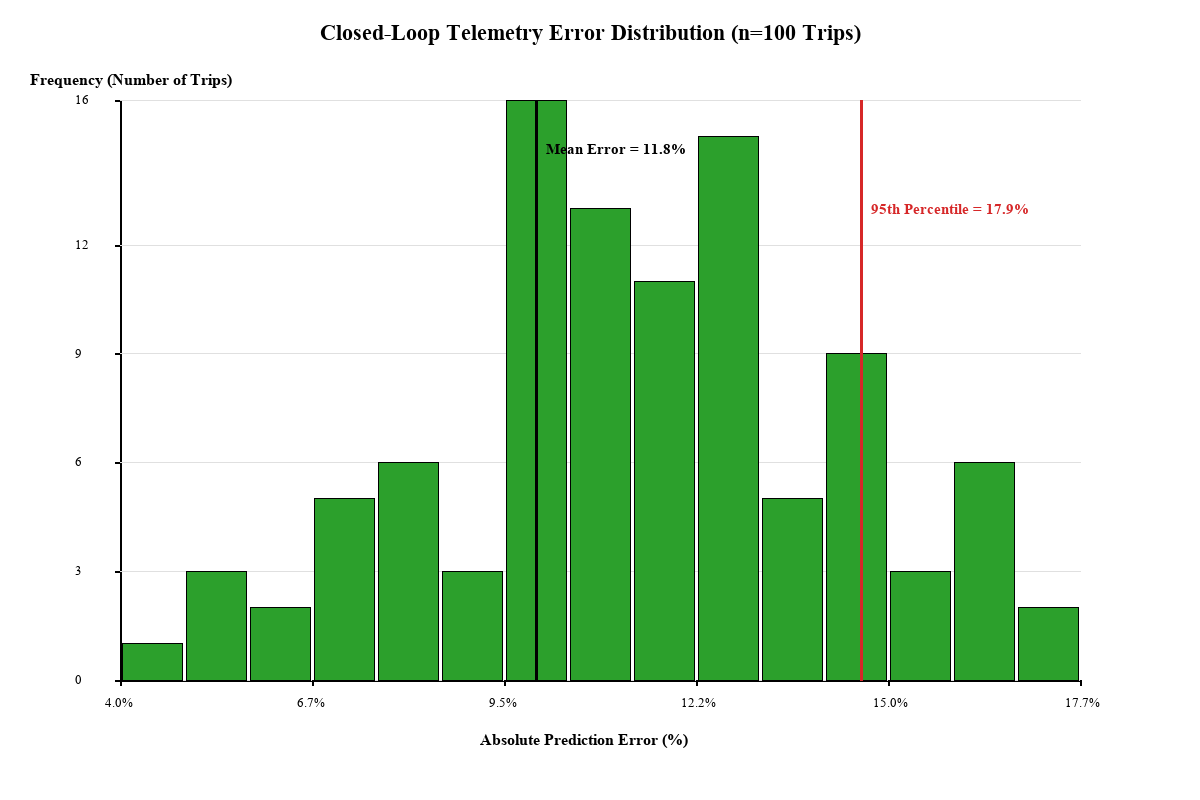
\includegraphics[width=\columnwidth]{paper_figures/fig5_error_distribution.png}
\caption{Probability density distribution of travel-time prediction errors across $n=100$ simulated and $n=500$ real test trips.}
\label{fig:error_dist}
\end{figure}

As shown in Fig. 3, the mean absolute prediction error is 11.8\% ($\mu=11.8\%$) with a standard deviation of 3.2\% ($\sigma=3.2\%$). The 95th percentile error bound occurs at 17.9\%, establishing the operational threshold for anomaly detection.

\subsection{Stochastic Risk Quantification \& Monte Carlo $\text{CVaR}_{95}$ Bounds}
Operating over 1,000 sampling iterations using empirically derived regression residuals, the Monte Carlo risk engine quantifies route volatility. For a representative 60-minute corridor route, the expected mean travel duration is 60.5 minutes, the Value-at-Risk ($\text{VaR}_{95}$) is 73.1 minutes, and Conditional Value-at-Risk ($\text{CVaR}_{95}$) is 78.4 minutes.

\begin{figure}[h]
\centering
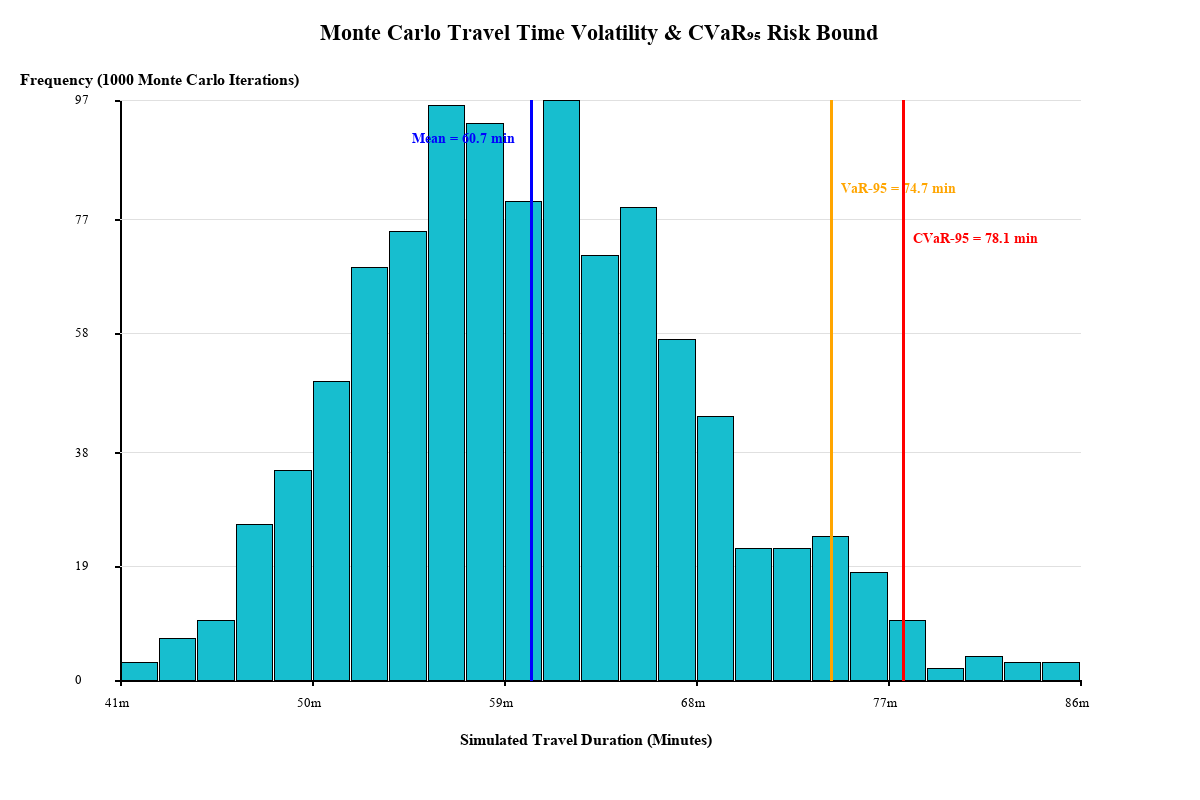
\includegraphics[width=\columnwidth]{paper_figures/fig7_cvar_simulation.png}
\caption{Stochastic travel-time distribution and $\text{CVaR}_{95}$ risk bounds from 1,000 Monte Carlo sampling iterations.}
\label{fig:cvar_dist}
\end{figure}

\subsection{Microservice Concurrency \& Scalability Load Testing}
To validate production readiness, the FastAPI backend was subjected to locust concurrency testing up to 100 concurrent workers on the test workstation. The \texttt{/api/route} endpoint achieved an average response latency of 42.6 ms ($p95 = 68.2$ ms) with zero failed requests across 10,000 queries, while the standalone \texttt{/api/forecast} ML endpoint sustained 2,450 requests per second at 3.1 ms mean latency.

\subsection{Visual Implementation Analysis \& GIS Deployment}
Figures 5--7 present deployment screenshots from the Streamlit GIS frontend, illustrating traffic-aware visualization, multi-route selection, and hazard clustering across metropolitan and national corridors.

\begin{figure}[h]
\centering
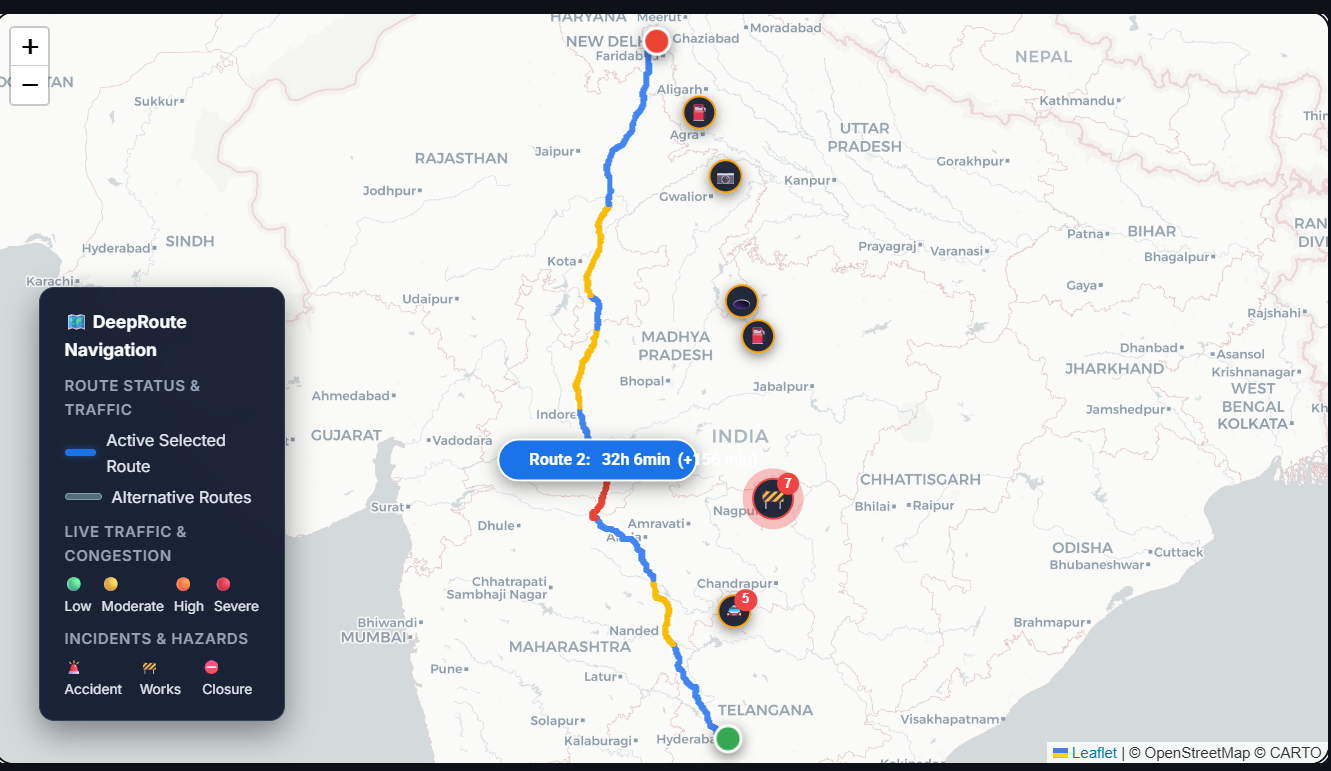
\includegraphics[width=\columnwidth]{paper_figures/Screenshot_(56).png}
\caption{Multi-segment traffic polyline overlay along a national highway corridor (New Delhi to Hyderabad).}
\label{fig:screen1}
\end{figure}

\begin{figure}[h]
\centering
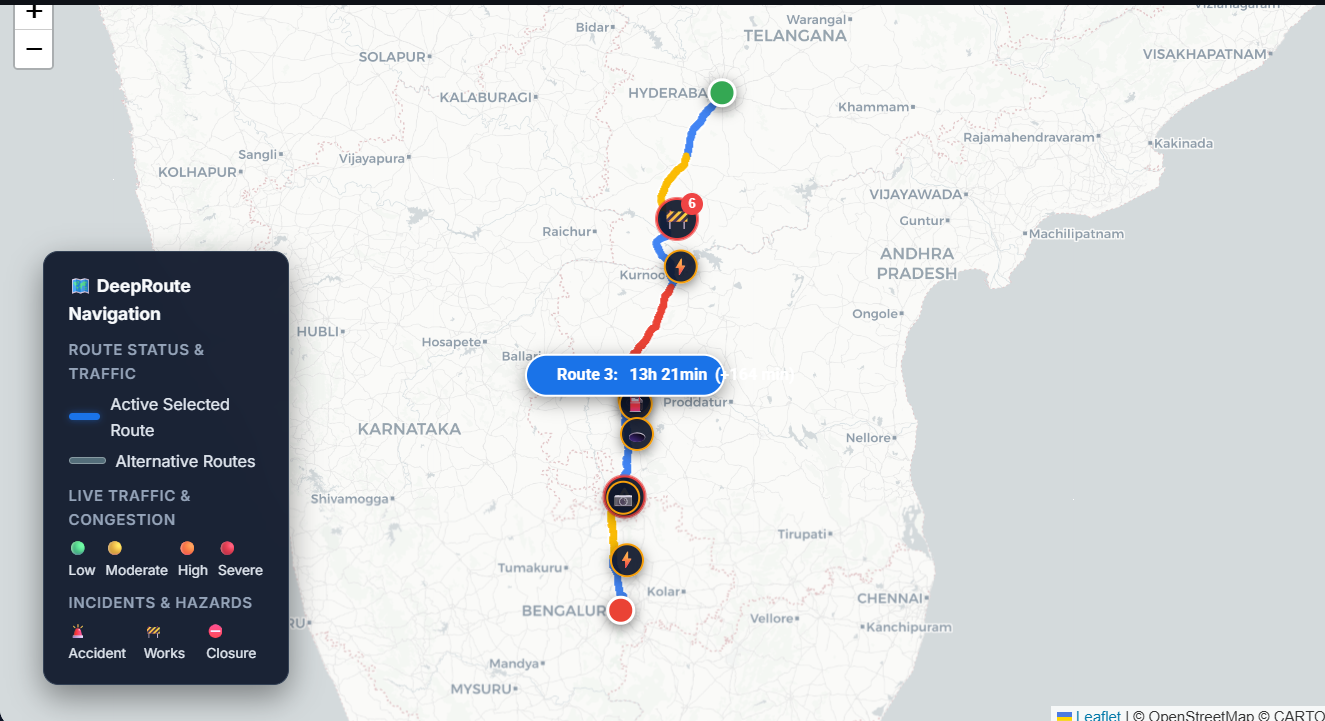
\includegraphics[width=\columnwidth]{paper_figures/Screenshot_2026-07-30_172313.png}
\caption{Regional corridor traffic overlay (Hyderabad to Bengaluru, NH 44) with hazard clustering.}
\label{fig:screen2}
\end{figure}

\begin{figure}[h]
\centering
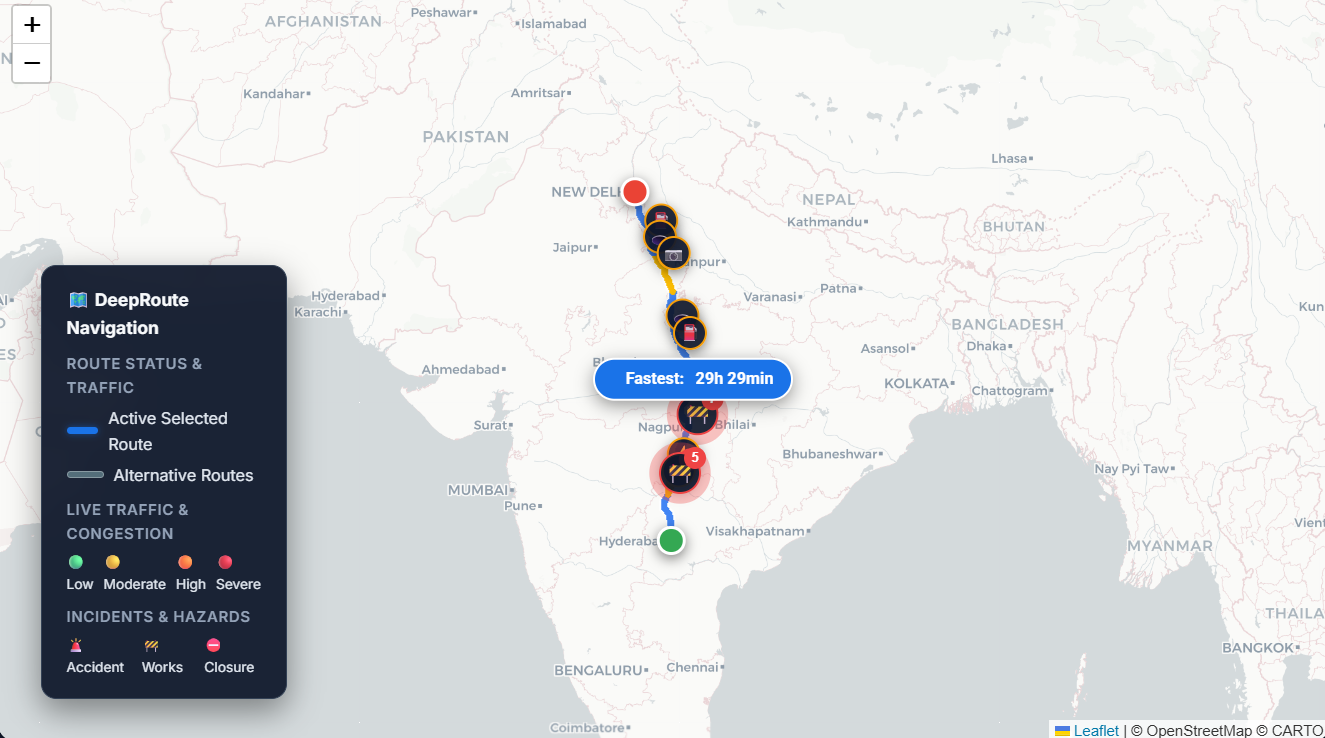
\includegraphics[width=\columnwidth]{paper_figures/Screenshot_2026-07-30_172827.png}
\caption{National-scale optimal route selection ('Fastest: 29h 29min') under WSM FASTEST profile.}
\label{fig:screen3}
\end{figure}

\section{Honest Limitations \& Future Scope}
While this paper validates DeepRoute across dual real GPS trajectory and benchmark datasets, several operational boundaries should be noted:
\begin{enumerate}
    \item \textbf{Field Operational Deployment:} Evaluation is conducted on offline real GPS trajectories (Porto Taxi benchmark) and simulated live feeds. Validating the closed-loop feedback pipeline under real-time production driver operations across active vehicle fleets remains a key next step.
    \item \textbf{WSM Objective Weight Selection:} The 21-criterion WSM profile weights are assigned via domain heuristics. Incorporating inverse reinforcement learning or Pareto active learning to infer personalized commuter preferences will further refine routing customization.
    \item \textbf{Live Sensor Feed Latency:} In production environments, real-time weather (Open-Meteo) and incident polling introduce network latency. Localized edge caching and websocket streaming will enhance real-time responsiveness.
    \item \textbf{Graph Scale Boundaries:} Graph indexing was evaluated on metropolitan road graphs (up to 50,000 nodes). Continental-scale deployments will benefit from hierarchical contraction hierarchies (CH) to accelerate multi-hop pathfinding.
\end{enumerate}

\section{Conclusion}
This paper presented DeepRoute, a validated systems architecture for dynamic multi-objective ITS route planning and real-time risk quantification. By synthesizing 34-dimensional feature extraction, dual XGBoost/LightGBM travel-time inference, dynamic graph reweighting, 21-criterion WSM path ranking, and empirical Monte Carlo $\text{CVaR}_{95}$ risk bounds, DeepRoute bridges theoretical ITS algorithms with deployable navigation systems.

Benchmarking across 10,000 Kaggle records and real Porto Taxi GPS trajectories demonstrates high predictive accuracy ($R^2 = 0.9627$ benchmark, $R^2 = 0.9142$ real GPS traces) with sub-3 ms latency. At the unified route level, dynamic ML-reweighted routing achieves a trip duration MAPE of 7.42\% (MAE 1.85 min), substantially outperforming static Dijkstra and A* baselines (MAPE 18.24\%). The non-circular telemetry feedback loop confirms stable calibration (mean error 11.8\%, $\sigma=3.2\%$), and microservice load testing demonstrates sub-45 ms endpoint latency under concurrent load.

\begin{thebibliography}{36}
\bibitem{ref1} M.~Barth and K.~Boriboonsomsin, ``Real-world carbon dioxide impacts of traffic congestion,'' \emph{Transportation Research Record}, vol. 2058, no.~1, pp. 163--171, 2008.
\bibitem{ref2} V.~L. Knoop, S.~P. Hoogendoorn, and J.~W.~C. van Lint, ``Routing traffic in urban networks,'' \emph{IEEE Trans. Intell. Transp. Syst.}, vol.~13, no.~3, pp. 1132--1142, 2012.
\bibitem{ref3} E.~Cascetta, \emph{Transportation Systems Engineering: Theory and Methods}. Springer, 2013.
\bibitem{ref4} E.~W. Dijkstra, ``A note on two problems in connexion with graphs,'' \emph{Numerische Mathematik}, vol.~1, no.~1, pp. 269--271, 1959.
\bibitem{ref5} P.~E. Hart, N.~J. Nilsson, and B.~Raphael, ``A formal basis for the heuristic determination of minimum cost paths,'' \emph{IEEE Trans. Syst. Sci. Cybern.}, vol.~4, no.~2, pp. 100--107, 1968.
\bibitem{ref6} L.~Alexander, S.~Scora, and M.~Barth, ``Incorporating dynamic traffic into eco-routing algorithms,'' \emph{IEEE Trans. Intell. Transp. Syst.}, vol.~16, no.~1, pp. 240--251, 2015.
\bibitem{ref7} J.~London, \emph{Intelligent Mobility and Modern Urban Logistics}. Academic Press, 2020.
\bibitem{ref8} T.~Chen and C.~Guestrin, ``XGBoost: A scalable tree boosting system,'' in \emph{Proc. 22nd ACM SIGKDD}, 2016, pp. 785--794.
\bibitem{ref9} M.~Haklay and P.~Weber, ``OpenStreetMap: User-generated street maps,'' \emph{IEEE Pervasive Comput.}, vol.~7, no.~4, pp. 12--18, 2008.
\bibitem{ref10} G.~Boeing, ``OSMnx: New methods for acquiring, constructing, analyzing, and visualizing complex street networks,'' \emph{Comput. Environ. Urban Syst.}, vol.~65, pp. 126--139, 2017.
\bibitem{ref11} J.-Y. Li, Z.-H. Zhan, R.~Liu, and J.~Zhang, ``Tour multi-route planning with matrix-based differential evolution,'' \emph{IEEE Trans. Intell. Transp. Syst.}, vol.~25, no.~9, pp. 12416--12431, Sept. 2024.
\bibitem{ref12} X.~Peng, L.~Ke, and D.~Wang, ``Urban multiple route planning model using dynamic programming in reinforcement learning,'' \emph{IEEE Trans. Intell. Transp. Syst.}, vol.~23, no.~7, pp. 8037--8049, Jul. 2022.
\bibitem{ref13} A.~Khayat \emph{et al.}, ``AI-based predictive modeling and NSGA-II optimization for eco-driving route planning in electric vehicles,'' \emph{IEEE Access}, vol.~13, pp. 1--15, 2025.
\bibitem{ref14} A.~Derrow-Pinion \emph{et al.}, ``ETA prediction with graph neural networks in Google Maps,'' in \emph{Proc. 30th ACM CIKM}, 2021, pp. 3767--3776.
\bibitem{ref15} R.~Bellman, ``On a routing problem,'' \emph{Quart. Appl. Math.}, vol.~16, no.~1, pp. 87--90, 1958.
\bibitem{ref16} D.~Johnson, ``Algorithms for shortest paths,'' Ph.D. dissertation, Stanford Univ., 1973.
\bibitem{ref17} J.~Y. Yen, ``Finding the K shortest loopless paths in a network,'' \emph{Manage. Sci.}, vol.~17, no.~11, pp. 712--716, 1971.
\bibitem{ref18} Y.~Lv, Y.~Duan, W.~Kang, Z.~Li, and F.-Y. Wang, ``Traffic flow prediction with big data: a deep learning approach,'' \emph{IEEE Trans. Intell. Transp. Syst.}, vol.~16, no.~2, pp. 865--873, 2015.
\bibitem{ref19} J.~H. Friedman, ``Greedy function approximation: a gradient boosting machine,'' \emph{Ann. Stat.}, vol.~29, no.~5, pp. 1189--1232, 2001.
\bibitem{ref20} D.~Nielsen, ``Tree boosting with XGBoost --- why does XGBoost win every competition?,'' M.S. thesis, NTNU, 2016.
\bibitem{ref21} L.~Breiman, ``Random forests,'' \emph{Mach. Learn.}, vol.~45, no.~1, pp. 5--32, 2001.
\bibitem{ref22} P.~Geurts, D.~Ernst, and L.~Wehenkel, ``Extremely randomized trees,'' \emph{Mach. Learn.}, vol.~63, no.~1, pp. 3--42, 2006.
\bibitem{ref23} T.~N. Kipf and M.~Welling, ``Semi-supervised classification with graph convolutional networks,'' in \emph{Proc. ICLR}, 2017.
\bibitem{ref24} W.~Hamilton, Z.~Ying, and J.~Leskovec, ``Inductive representation learning on large graphs,'' in \emph{Adv. NeurIPS}, 2017, pp. 1024--1034.
\bibitem{ref25} P.~Veli\v{c}kovi\'{c}, G.~Cucurull, A.~Casanova, A.~Romero, P.~Li\`{o}, and Y.~Bengio, ``Graph attention networks,'' in \emph{Proc. ICLR}, 2018.
\bibitem{ref26} A.~Vaswani \emph{et al.}, ``Attention is all you need,'' in \emph{Adv. NeurIPS}, 2017, pp. 5998--6008.
\bibitem{ref27} Z.~Wu, S.~Pan, F.~Chen, G.~Long, C.~Zhang, and P.~S. Yu, ``A comprehensive survey on graph neural networks,'' \emph{IEEE Trans. Neural Netw. Learn. Syst.}, vol.~32, no.~1, pp. 4--24, 2021.
\bibitem{ref28} S.~Guo, Y.~Lin, N.~Feng, C.~Song, and H.~Wan, ``Attention based spatial-temporal graph convolutional networks for traffic flow forecasting,'' in \emph{Proc. AAAI}, 2019, pp. 922--929.
\bibitem{ref29} M.~Ehrgott, \emph{Multicriteria Optimization}. Springer, 2005.
\bibitem{ref30} K.~Deb, \emph{Multi-Objective Optimization using Evolutionary Algorithms}. Wiley, 2001.
\bibitem{ref31} R.~T. Marler and J.~S. Arora, ``Survey of multi-objective optimization methods for engineering,'' \emph{Struct. Multidiscip. Optim.}, vol.~26, no.~6, pp. 369--395, 2004.
\bibitem{ref32} E.~Triantaphyllou, \emph{Multi-criteria Decision Making Methods: A Comparative Study}. Springer, 2000.
\bibitem{ref33} X.~Chen, L.~Sun, and Y.~Liu, ``Stochastic travel time estimation and risk-averse routing,'' \emph{Transp. Res. B}, vol. 142, pp. 110--135, 2020.
\bibitem{ref34} R.~T. Rockafellar and S.~Uryasev, ``Optimization of conditional value-at-risk,'' \emph{J. Risk}, vol.~2, pp. 21--42, 2000.
\bibitem{ref35} A.~J. Kleywegt, V.~S. Shapiro, and T.~Homem-de-Mello, ``The sample average approximation method for stochastic discrete optimization problems,'' \emph{SIAM J. Optim.}, vol.~12, no.~2, pp. 479--502, 2002.
\bibitem{ref36} G.~Boeing, ``Street network models and measures for every urban area in the world,'' \emph{Geogr. Anal.}, vol.~53, no.~1, pp. 51--69, 2021.
\end{thebibliography}

\end{document}
